\section*{Appendix}

\subsection{Detailed construction of $\hat{\M}_{sub}^\times$}

Recall that we split the set of accepting states ${\acc}^\times$ into two virtual copies: i) $I_{in}$, which only has incoming transitions into
${\acc}^\times$, and ii) $I_{out}$, which only has outgoing transitions from ${\acc}^\times$. Then the new state-space can be defined as 
\begin{equation*}
    \hat{S}:=(S_p \setminus {\acc}^\times)\cup I_{in}\cup I_{out}
\end{equation*}

Over $\hat S$, one can further construct a new product MDPST 
\begin{equation}\label{def:hat_mdpst}
    \hat{\mathcal{M}}^\times_{sub}=(\hat{S}, s^\times_{0}, \hat{A}^{\times}, \hat{\mathcal{F}}^{\times},  \hat{\mathcal{T}}^{\times}, \hat{\mathcal{L}}^{\times}),
\end{equation}
where 
\begin{itemize}
    \item $\hat{A}^{\times}=A^\times\cup \{\tau_0\}$ and $\tau_0$ is a self-loop action. The set of available actions $\hat{A}^{\times}(s)$ is defined as $\hat{A}^{\times}(s)=A^\times(s), \forall s\in S_p \setminus \acc^\times$, $\hat{A}^{\times}(s^{\rm out})=A^\times(s), \forall s \in \acc^\times$, and $\hat{A}^{\times}(s^{\rm in})=\tau_0, \forall s\in \acc^\times$, where $s^{\rm out}$ and $s^{\rm in}$ are respectively the virtual copies of $s\in \acc^\times$ in $I_{in}$ and $ I_{out}$.
    \item $\hat{\F}^{\times}: \hat{S} \times \hat{A}^{\times} \Mapsto 2^{2^{\hat{S}^\times}}$ is the set-valued nondeterministic transition function. To define $\hat{\F}^{\times}$, we let $\Phi = \cup_{s\in S_p}\cup_{a\in {A}^{\times}} \cup_{\Theta\in \F_p(s, a)}\{\Theta\}$ be the set of all possible target (single- or set-valued) states originating from ${S}_p$. For each set $\Theta \in \Phi$, we define a \emph{copy} $\hat{\Theta}$ of $\Theta$ as i) $\hat{\Theta} = \Theta$ if $\Theta \subseteq S_p \setminus \acc^\times$, ii) $\hat{\Theta} = \{s^{\rm in}: s\in \Theta\}$ if $\Theta \subseteq \acc^\times$, and iii) $\hat{\Theta} = \{s: s\in \Theta \wedge s\in S_p \setminus \acc^\times\} \cup \{s^{\rm in}: s\in \Theta \wedge s \in \acc^\times\}$, otherwise. Then, one has that
    \begin{itemize}
        \item if $s\in S_p\setminus \acc^\times$, $\hat{\Theta} \in \hat{\F}^{\times}(s, a) \ \text{iff} \ \Theta \in \F_p(s, a)$;
        \item if $s^{\rm out}\in I_{out}$, $\hat{\Theta} \in \hat{\F}^{\times}(s^{\rm out}, a) \ \text{iff} \ \Theta \in \F_p(s, a)$;
        \item if $s^{\rm in}\in I_{in}$, $\hat{\F}^{\times}(s^{\rm in}, \tau_0) = s^{\rm in}$.
    \end{itemize}
   \item  $\hat{\mathcal{T}}^{\times}: \hat{S}\times \hat{A}^{\times} \times {2^{\hat{S}^\times}}\mapsto (0, 1]$ is the transition probability function, given by
   \begin{itemize}
       \item $\hat{\mathcal{T}}^{\times}(s, a, \hat{\Theta})= \mathcal{T}_p(s, a, {\Theta})$ for $s\in S_p\setminus \acc^\times$,
       \item $\hat{\mathcal{T}}^{\times}(s^{\rm out}, a, \hat{\Theta})= \mathcal{T}_p(s, a, {\Theta})$ for $s^{\rm out}\in I_{out}$,
       \item $\hat{\mathcal{T}}^{\times}(s^{\rm in}, \tau_0, s^{\rm in})= 1$ for $s^{\rm in}\in I_{in}$.       
   \end{itemize}
   \item $\hat{\L}^{\times}: \hat{S} \to 2^{Prop}$, where $\hat{\L}^{\times}(s)=\L^\times(s)$ if $s\in S_p\setminus \acc^\times$ and $\hat{\L}^{\times}(s^{\rm out})=\hat{\L}^{\times}(s^{\rm in})=\L^\times(s)$ otherwise.
\end{itemize}

Note that $\hat{\mathcal{M}}^\times_{sub}$ is equivalent to ${\M}^\times_{sub}$ in the sense that there exists a one-to-one correspondence between the transitions of $\hat{\mathcal{M}}^\times_{sub}$ and ${\M}^\times_{sub}$. 

\subsection{Example for demonstrating Algorithm 1}

\begin{example}
    Consider a product MDPST ${\M}^\times$ with the set of states $S^\times = \{S_1, \cdots, S_{10}\}$ and the set of actions $A^\times = \{a, b\}$, as shown in Fig. {\ref{fig:mdpst_v1}}. The initial state is $s_0^\times = S_1$ and the set of accepting states is given by $\acc^\times = \{S_4, S_5\}$ (marked in green). For the state $S_2$, both actions $a$ and $b$ are applicable and the associated (action labelled) probabilistic transitions are depicted. For the remaining states, only action $a$ is applicable and the associated  probabilistic transitions are depicted (where the action label is omitted). Notice that state $S_{10}$ is not backward reachable from the set of accepting states $\acc^\times$, therefore it follows that $S_p = \{S_1, \cdots, S_{9}\}$ and the resulting sub-MDPST ${\M}^\times_{sub}$ is shown within the shaded box of Fig. {\ref{fig:mdpst_v1}}.

    In the first iteration of Algorithm 1, one starts by splitting $\acc^\times$ into two virtual copies of $I_{in}= \{S_4^{in}, S_5^{in}\}$ and $I_{out}= \{S_4^{out}, S_5^{out}\}$. Then the new state space $\hat{S} = \{S_1, \cdots, S_3, S_4^{in}, S_5^{in}, S_4^{out}, S_5^{out}, S_6, \cdots, S_9\}$ and the constructed MDPST $\hat{\M}^\times_{sub}$ is drawn in Fig. \ref{fig:mdpst_v2}. Let $V_{sat}(S_4^{in})=V_{sat}(S_5^{in}) = 1$. With the robust dynamic programming operator $T$ in (\ref{VF_deterministic}), one can compute that $V_{sat}(S_1)=0.8, V_{sat}(S_2) = V_{sat}(S_3) = V_{sat}(S_4^{out}) = 1$, $V_{sat}(S_5^{out})= V_{sat}(S_6) = V_{sat}(S_7) = V_{sat}(S_8) = 0$, and $V_{sat}(S_9) = 0.94$. Therefore, we remove state $S_5$ from both $\acc^{\times}$ and $S_p$, and further remove states $S_1, S_6, S_7, S_8, S_9$ from $S_p$, and thus obtain $S_p = \{S_2, S_3, S_4\}$ and $\acc^{\times} = \{S_4\}$ for the second iteration.

    The product MDPST ${\M}^\times_{sub}$ for the second iteration is depicted in Fig. \ref{fig:WR}. By repeating the process in iteration 1, one can get that $V_{sat}(S_2) = V_{sat}(S_3) = V_{sat}(S_4^{in}) = V_{sat}(S_4^{out}) = 1$. Thus, one has that flag$=0$. The iteration terminates. The WR is then given by $W^\times = \{S_2, S_3, S_4\}$.
\end{example}

\begin{figure}[ht]
\centering
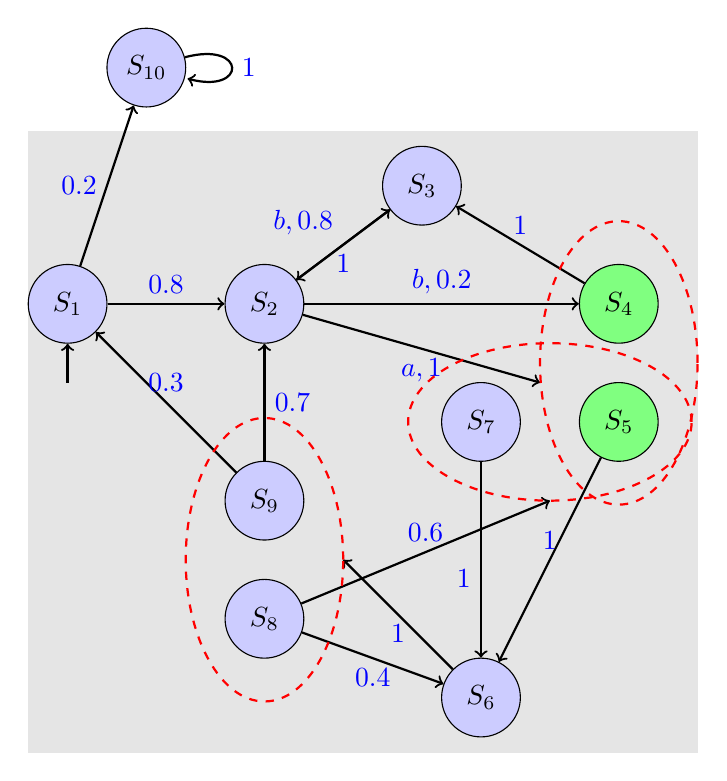
\begin{tikzpicture}

\fill[gray!20] (0, -5.7) rectangle (8.5, 2.2);
% Define states (S1, S2, S3, ... S10)
\node[circle, draw, fill=blue!20, minimum width=1cm, minimum height=0.5cm] (S1) at (0.5, 0) {$S_1$};
\node[circle, draw, fill=blue!20, minimum width=1cm, minimum height=0.5cm] (S2) at (3, 0) {$S_2$};
\node[circle, draw, fill=blue!20, minimum width=1cm, minimum height=0.5cm] (S3) at (5, 1.5) {$S_3$};
\node[circle, draw, fill=green!50, minimum width=1cm, minimum height=0.5cm] (S4) at (7.5, 0) {$S_4$};
\node[circle, draw, fill=green!50, minimum width=1cm, minimum height=0.5cm] (S5) at (7.5, -1.5) {$S_5$};
\node[circle, draw, fill=blue!20, minimum width=1cm, minimum height=0.5cm] (S6) at (5.75, -5) {$S_6$};
\node[circle, draw, fill=blue!20, minimum width=1cm, minimum height=0.5cm] (S7) at (5.75, -1.5) {$S_7$};
\node[circle, draw, fill=blue!20, minimum width=1cm, minimum height=0.5cm] (S8) at (3, -2.5) {$S_9$};
\node[circle, draw, fill=blue!20, minimum width=1cm, minimum height=0.5cm] (S9) at (3, -4) {$S_8$};
\node[circle, draw, fill=blue!20, minimum width=1cm, minimum height=0.5cm] (S10) at (1.5, 3) {$S_{10}$};


% Transitions (arrows with weights)
\draw[->, thick] (S1) -- node[midway, left, blue] {$0.2$} (S10); % Edge to the group
\draw[->, thick] (S1) -- node[midway, above, blue] {$0.8$} (S2); % Edge to the group
\draw[->, thick] (S2) -- node[midway, above, blue] {$b, 0.2$} (S4); % Edge to the group
\draw[->, thick] (S2) -- node[midway, above left, blue] {$b, 0.8$} (S3);
\draw[->, thick] (S2) -- node[midway, below, blue] {$a, 1$} (6.5, -1);
\draw[->, thick] (S3) -- node[midway, below, blue] {1} (S2); % Edge to the group
\draw[->, thick] (S4) -- node[midway, above, blue] {1} (S3); % Edge to the group
\draw[->, thick] (S5) -- node[midway, above, blue] {1} (S6); % Edge to the group
\draw[->, thick] (S6) -- node[midway, below, blue] {1} (4, -3.25);
\draw[->, thick] (S7) -- node[midway, below left, blue] {1} (S6);
\draw[->, thick] (S9) -- node[midway, above, blue] {0.6} (6.625, -2.5);
\draw[->, thick] (S9) -- node[midway, below, blue] {0.4} (S6);
\draw[->, thick] (S8) -- node[midway, above, blue] {0.3} (S1);
\draw[->, thick] (S8) -- node[midway, right, blue] {0.7} (S2);

\draw[->, thick] (.5, -1) -- (S1);


% Red dashed ellipse to group S2 and S3
\draw[red, dashed, thick] (7.5, -0.75) ellipse (1cm and 1.8cm);
\draw[red, dashed, thick] (6.625, -1.5) ellipse (1.8cm and 1cm);
\draw[red, dashed, thick] (3, -3.25) ellipse (1cm and 1.8cm);

\draw[->, thick] (S10) edge [loop right] node[right, blue] {1} (S10);
\end{tikzpicture}
\caption{The product MDPST $\M^\times$, where the sub-MDPST $\M_{sub}^\times$ (for the first iteration) is the part within the shaded box. }
\label{fig:mdpst_v1}
\end{figure}

\begin{figure}[t]
\centering
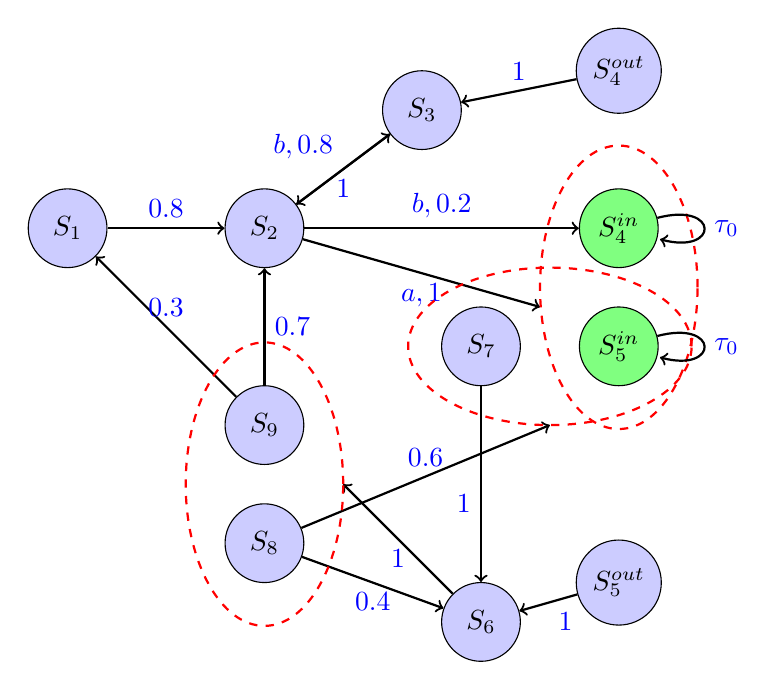
\begin{tikzpicture}

% Define states (S1, S2, S3, ... S9)
\node[circle, draw, fill=blue!20, minimum width=1cm, minimum height=0.5cm] (S1) at (0.5, 0) {$S_1$};
\node[circle, draw, fill=blue!20, minimum width=1cm, minimum height=0.5cm] (S2) at (3, 0) {$S_2$};
\node[circle, draw, fill=blue!20, minimum width=1cm, minimum height=0.5cm] (S3) at (5, 1.5) {$S_3$};
\node[circle, draw, fill=green!50, minimum width=1cm, minimum height=0.5cm] (S4) at (7.5, 0) {$S_4^{in}$};
\node[circle, draw, fill=blue!20, minimum width=1cm, minimum height=0.5cm] (S42) at (7.5, 2) {$S_4^{out}$};
\node[circle, draw, fill=green!50, minimum width=1cm, minimum height=0.5cm] (S5) at (7.5, -1.5) {$S_5^{in}$};
\node[circle, draw, fill=blue!20, minimum width=1cm, minimum height=0.5cm] (S52) at (7.5, -4.5) {$S_5^{out}$};
\node[circle, draw, fill=blue!20, minimum width=1cm, minimum height=0.5cm] (S6) at (5.75, -5) {$S_6$};
\node[circle, draw, fill=blue!20, minimum width=1cm, minimum height=0.5cm] (S7) at (5.75, -1.5) {$S_7$};
\node[circle, draw, fill=blue!20, minimum width=1cm, minimum height=0.5cm] (S8) at (3, -2.5) {$S_9$};
\node[circle, draw, fill=blue!20, minimum width=1cm, minimum height=0.5cm] (S9) at (3, -4) {$S_8$};


% Transitions (arrows with weights)
\draw[->, thick] (S1) -- node[midway, above, blue] {$0.8$} (S2); % Edge to the group
\draw[->, thick] (S2) -- node[midway, above, blue] {$b, 0.2$} (S4); % Edge to the group
\draw[->, thick] (S2) -- node[midway, above left, blue] {$b, 0.8$} (S3);
\draw[->, thick] (S2) -- node[midway, below, blue] {$a, 1$} (6.5, -1);
\draw[->, thick] (S3) -- node[midway, below, blue] {1} (S2); % Edge to the group
\draw[->, thick] (S42) -- node[midway, above, blue] {1} (S3); % Edge to the group
\draw[->, thick] (S52) -- node[midway, below right, blue] {1} (S6); % Edge to the group
\draw[->, thick] (S6) -- node[midway, below, blue] {1} (4, -3.25);
%\draw[->, thick] (S7) -- node[midway, above, blue] {0.5} (S8);
\draw[->, thick] (S7) -- node[midway, below left, blue] {1} (S6);
\draw[->, thick] (S9) -- node[midway, above, blue] {0.6} (6.625, -2.5);
\draw[->, thick] (S9) -- node[midway, below, blue] {0.4} (S6);
\draw[->, thick] (S8) -- node[midway, above, blue] {0.3} (S1);
\draw[->, thick] (S8) -- node[midway, right, blue] {0.7} (S2);


% Red dashed ellipse to group S2 and S3
\draw[red, dashed, thick] (7.5, -0.75) ellipse (1cm and 1.8cm);
\draw[red, dashed, thick] (6.625, -1.5) ellipse (1.8cm and 1cm);
\draw[red, dashed, thick] (3, -3.25) ellipse (1cm and 1.8cm);

\draw[->, thick] (S4) edge [loop right] node[right, blue] {$\tau_0$} (S4);
\draw[->, thick] (S5) edge [loop right] node[right, blue] {$\tau_0$} (S5);

%\draw[->, thick] (.5, -1) -- (S1);

\end{tikzpicture}
\caption{The constructed product MDPST $\hat{\M}_{sub}^\times$.} \label{fig:mdpst_v2}
\end{figure}



\begin{figure}[t]
\centering
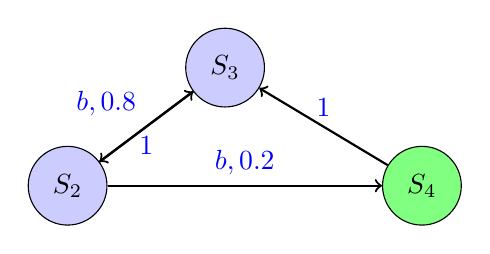
\begin{tikzpicture}

% Define states (S1, S2, S3, ... S9)
\node[circle, draw, fill=blue!20, minimum width=1cm, minimum height=0.5cm] (S2) at (3, 0) {$S_2$};
\node[circle, draw, fill=blue!20, minimum width=1cm, minimum height=0.5cm] (S3) at (5, 1.5) {$S_3$};
\node[circle, draw, fill=green!50, minimum width=1cm, minimum height=0.5cm] (S4) at (7.5, 0) {$S_4$};


% Transitions (arrows with weights)
\draw[->, thick] (S2) -- node[midway, above, blue] {$b, 0.2$} (S4); % Edge to the group
\draw[->, thick] (S2) -- node[midway, above left, blue] {$b, 0.8$} (S3);
\draw[->, thick] (S3) -- node[midway, below, blue] {1} (S2); % Edge to the group
\draw[->, thick] (S4) -- node[midway, above, blue] {1} (S3); % 
\end{tikzpicture}
\caption{The product MDPST $\M_{sub}^\times$ for the second iteration.}
\label{fig:WR}
\end{figure}

\subsection{Proof of Theorem \ref{thm1}}
% \pian{@yong, please double check the proof.}

We prove Theorem \ref{thm1} in two steps. 

\paragraph{Step 1} We show the correctness of Algorithm 1, i.e., that the output $W^\times$ of Algorithm 1 is indeed the WR of the product MDPST $\M^\times$. More specifically, for every state $s^\times\in W^{\times}$, we have that 
    \begin{itemize}
        \item there exists a strategy $\sigma^\times$ from $s^\times$ such that $\prob_{{\mathcal{M}^\times}}^{\sigma^\times(s^\times)}(\square\diamondsuit \acc^{\times}) = 1$.
    \end{itemize}

    First, for a state $s^\times \in W^{\times}$, $\prob_{{\mathcal{M}^\times}}^{\sigma^\times(s^\times)}(\diamondsuit \acc^{\times}) = 1$, since $\hat{V}_{sat}(s^\times) = 1$, which means that there exists a strategy starting from $s^\times$ and leading to the virtual copies of accepting states in $I_{in}$ with probability one.
    If $s \in W^{\times}$, there must be the virtual copies of accepting states in $I_{out}$ that belong to $W^{\times}$, otherwise those states $s^{out} \in I_{out}$ will be removed from $\acc^{\times}$ (cf. line 10).
    Since $s \in W^{\times}$, we have a strategy $\sigma_1$ to generate a run from $s$ reaching an accepting state, say $s^{in}_1 \in I_{in}$, against any nature $\gamma$.
    Then we know that the virtual copy $s^{out}_1 \in I_{out}$ also belongs to $W^{\times}$, otherwise the accepting state $s_1$ will be removed from $\acc^{\times}$ (cf. line 10).
    As a result, there exists a strategy $\sigma_2$ to generate a run from $s^{out}_1$ (and thus $s_1$) to an accepting state $s^{in}_2\in I_{in}$ against any nature $\gamma$ with probability one.
    Similarly, from $s^{out}_2$, we can extend the run to another accepting state $s^{in}_3$, and so on.
    Since the number of accepting states in $W^{\times}$ is finite, there must be an accepting state that is visited infinitely often.
    Hence, by merging the virtual copies of accepting states into their original state in this generated run, we can obtain an accepting run in $\M^{\times}$.
    Moreover, the probability measure of this run is $1$, as each constructed fragment run has probability measure $1$.
    By combining all these strategies $\sigma_1, \sigma_2, \cdots, \sigma_n$ constructed up to the point where the nature $\gamma$ has repeated its behavior as it only has finite memory, we can obtain the strategy $\sigma = \sigma_1 \cdot \sigma_2 \cdots \sigma_n$.
    It immediately follows that $\prob_{{\mathcal{M}^\times}}^{\sigma^\times(s^\times)}(\square\diamondsuit \acc^{\times}) = 1$.

As long as a run gets trapped in the WR, we have a strategy to keep the run in the WR with probability one.
It immediately follows that:
\begin{equation*}
    \begin{aligned}
        \max\limits_{{\sigma^\times}\in {\Pi_{{\M}^\times}}} \{\prob_{{\M}^\times}^{{{\sigma^\times}}}( \diamondsuit \square W^\times)\} &= \max\limits_{{\sigma^\times}\in {\Pi_{{\M}^\times}}} \{\prob_{{\M}^\times}^{{{\sigma^\times}}}( \diamondsuit W^\times)\}\\
    &= \max\limits_{{\sigma^\times}\in {\Pi_{{\M}^\times}}} \{\prob_{{\M}^\times}^{{{\sigma^\times}}}( \diamondsuit \square \acc^\times)\}.
    \end{aligned}
\end{equation*}

\paragraph{Step 2} We show that
\begin{equation*}
    \max\limits_{\sigma\in \Pi_{\M}}\{\prob_{{\M}}^\sigma(\varphi)\}
        = \max\limits_{{\sigma^\times}\in {\Pi_{{\M}^\times}}} \{\prob_{{\M}^\times}^{{{\sigma^\times}}}( \diamondsuit \square W^\times)\}
\end{equation*}
holds by verifying both sides of the inequality and subsequently constructing the induced policy on $\M$.

Let $p = \max_{\sigma} \{ {\rm Pr}_{{\mathcal{M}}}^\sigma(\varphi) \}$. In other words, there is an \emph{optimal} robust strategy $\sigma$ such that, for every possible nature $\gamma$ of $\mathcal{M}$, we have ${\rm Pr}_\mathcal{M}^{\sigma, \gamma}(\varphi) \geq p$ and there exists some nature $\gamma'$ such that ${\rm Pr}_\mathcal{M}^{\sigma, \gamma'}(\varphi) = p$.
For every fixed strategy $\sigma$ and nature $\gamma$, we can obtain a Markov chain $\mathcal{M}_{\sigma,\gamma}$.

To prove the direction of $\leq$, we will construct a strategy $\sigma^{\times}$ for $\mathcal{M}^{\times}$ such that, for every nature $\gamma^{\times}$, ${\prob^{\sigma^{\times}, \gamma^{\times}}_{\mathcal{M}^{\times}}(\diamondsuit \square W^{\times})} \geq p$.
Observe that every nature $\gamma^{\times}$ for $\mathcal{M}^{\times}$ induces a nature $\gamma$ for $\mathcal{\M}$ by ignoring the component from the automaton $\mathcal{\A}$.
Both Markov chains $\mathcal{M}_{\sigma, \gamma}$ and $\mathcal{M^{\times}_{\sigma^{\times}, \gamma^{\times}}}$ (ignoring the acceptance condition) will have the same probability to generate traces that satisfy $\varphi$, because the probability in $\mathcal{M}^{\times}$ comes only from $\mathcal{M}$.
Thus, for every nature $\gamma^{\times}$ we construct $\sigma^{\times}$ by following $\sigma$ of $\mathcal{M}$ within the state space $S \times Q_i$ and $S \times Q_{acc}$, where $Q_{i}$ (respectively, $Q_{acc}$) is the deterministic part of $Q$ before (respectively, after) seeing an $\epsilon$-transition.
This is possible because the automaton transitions within $Q_i$ and $Q_{acc}$ separately are deterministic.
To resolve the nondeterministic jump from $Q_i$ to $Q_{acc}$ (i.e., $\epsilon$-transitions), we select the automaton successors according to the behavior of the Markov chain $\M_{\sigma, \gamma}$.
That is, before $\M_{\sigma, \gamma}$ enters a bottom strongly connected component (BSCC), $\sigma^{\times}$ follows $\sigma$ in $\M$ and stays within the $Q_i$ part in $\aut$. 
The moment when $\M_{\sigma, \gamma}$ enters a BSCC from a product state $(s, q)$, according to \cite{sickert2016limit}, there is a way to select a successor $q'$ in $Q_{acc}$ for the state $q$ such that the trace generated by $\M_{\sigma, \gamma}$ from $(s, q)$ satisfies $\varphi$ if, and only if, the corresponding run from state $q'$ is accepted by $\aut$.
So, from state $(s, q)$, $\sigma^{\times}$ selects the action $\epsilon_{q'}$ and the run moves to $(s, q')$.
Afterwards, $\sigma^{\times}$ follows $\sigma$ in $\M$ and the run in $\aut$ is again deterministic.
We can see that $\sigma^{\times}$ basically imitates the behavior of $\sigma$ except for resolving the nondeterminism in the automaton $\aut$.
One can see that every trace $\rho$ in $\M_{\sigma, \gamma}$ corresponds to a trace $\rho^{\times}$ in $\M^{\times}_{\sigma^{\times}, \gamma^{\times}}$ with equal transition probabilities except for the $\epsilon$-transition, which has probability $1$.
Moreover, as aforementioned, if $\rho$ satisfies $\varphi$, the run $\rho^{\times}$, projected to the second component, is also an accepting run in $\aut$.

Now we only need to prove that the accepting trace $\rho^{\times}$ will stay within the WR $W^\times$ in the end.
Obviously, all states that occur in $\rho^{\times}$ infinitely many times, denoted $C$, can reach each other.
It must be the case that $C \subseteq W^{\times}$.
This is because the run $\rho^{\times}$ already enters a BSCC of $\M_{\sigma, \gamma}$ and the probability measure of this run in the BSCC is $1$.
Since $\rho$ is accepting, there must be an accepting state $s^{\times} \in \acc^{\times}$ that can visit itself with probability one under the strategy $\sigma$ against any adversarial nature $\gamma$.
Moreover, $s^{\times}$ clearly can be reached from the initial state.
Therefore, after applying Algorithm~1, $s^{\times}$ must belong to $W^{\times}$.
Since all states in the BSCC $C$ can reach accepting state $s^{\times}$ with probability one against any nature $\gamma$, we have that $C \subseteq W^{\times}$.
That is, the accepting run $\rho^{\times}$ eventually stays in $W^{\times}$. We then have that ${\prob^{\sigma^{\times}, \gamma^{\times}}_{\M^{\times}}(\diamondsuit \square W^{\times}) \geq \prob^{\sigma, \gamma}_{\mathcal{M}}(\varphi)} \geq p$ as $\sigma$ is an optimal robust strategy for $\M$.

The direction of $\geq$ is trivial. For any run that eventually stays within the WR $W^{\times}$, it will almost surely visit an accepting state infinitely many times.
Hence, the run must meet the B\"uchi condition.
It is clear that any strategy $\sigma^\times$ on $\M^\times$ can induce a policy for $\M$ by eliminating the $\epsilon$-transitions. Therefore, any path following $\sigma^\times$ that meets the B\"{u}chi condition will induce
a path of $\M$ that is accepting by $\A$ induced from $\varphi$, where the non-determinism of $\A$ is resolved by $\epsilon$-transitions of $\sigma^\times$, thus
satisfying $\varphi$.

Therefore, we have completed the proof.
%\end{proof}


% \begin{remark}
%     It is not trivial to show that LDBA is Good-for-MDPSTs (i.e., can be used for quantitative analysis of MDPSTs). This is mainly due to the additional unquantifiable uncertainty encoded in MDPSTs. In this work, we propose a novel notion called \emph{set-valued end component} for MDPSTs and an algorithm for computing accepting maximal SEC for the product MDPST $\m^\times$. By further eliminating the set-valued states in the accepting maximal SEC (they are not needed since MDPST is fully observable), we show that one can reduce the MDPST synthsis problem for \LTL to reachability problem over $\M^\times =\M \times \A$, where $\A$ is an LDBA and the set og goal states $G$ is given by (\ref{eqn:goal}).
% \end{remark}

% For $\le$, it has been proven in [Sickert et al., 2016] that, for every accepting path of an MDP following a policy $\delta$, there always exists a corresponding accepting run $\xi$ of the LDBA that resolves the non-determinism. This statement also holds for MDPSTs. This is because for every MDPST $\M = (S, s_0, A, \F, \T)$, one can construct a corresponding MDP $\M' = (S, s_0, A, \T')$, where for each set-valued transitions $\Theta \in \F(s, a)$ in MDPST, the (single-valued) transition function $\T'$ in MDP is given by $\T'(s, a, s') = \T(s, a, \Theta)/|\Theta|, \forall s'\in \Theta$. 
% \ly{Should be $\T'(s, a, s') = \Sigma_{\Theta \in \F(s, a), s'\in \Theta} \T(s, a, \Theta)/|\Theta|$ ?}
% It is straightforward to show that $\M$ and $\M'$ have the same set of paths given the same strategy. Augmenting the
% resolved non-determinism as $\epsilon$-actions to the original path yields an accepting path of $\M^\times$. This is because i) the SEC $\E$ of the  $\M^\times$ satisfies the EC properties, meaning that every element $\Theta$ in $\E$ is visited infinitely often with probability 1 and ii) according to our definition of AMSEC, one has that for each AMSEC $(\hat{\Xi}_k, A_k)$, there exists $\Theta\in \hat{\Xi}_k$ such that $\Theta \subseteq {\rm Acc}^\times$, this guarantees that at least one of the states in ${\rm Acc}^\times$ is visited infinitely often. Therefore, we have created a strategy for $\M^\times$ that is at least as good as on $\M$.

% For $\ge$, it is clear that any strategy $\sigma^\times$ on $\M^\times$ can induce a policy for $\M$ by eliminating the $\epsilon$-transitions. Therefore, any path following $\sigma^\times$ that meets the B\"{u}chi condition will induce
% a path of $\M$ that is accepting by $\A$ induced from $\varphi$, where the non-determinism of $\A$ is resolved by $\epsilon$-transitions of $\sigma^\times$, thus
% satisfying $\varphi$.


% \ly{Alternative proof}

% Let $p = \max_{\sigma} \{ {\rm Pr}_{{\mathcal{M}}}^\sigma(\varphi) \}$. In other words, there is an \emph{optimal} robust strategy $\sigma$ such that for every possible nature $\gamma$ of $\mathcal{M}$, we have ${\rm Pr}_\mathcal{M}^{\sigma, \gamma}(\varphi) \geq p$ and there exists some nature $\gamma'$ such that ${\rm Pr}_\mathcal{M}^{\sigma, \gamma}(\varphi) = p$.
% For every fixed strategy $\sigma$ and nature $\gamma$, we can obtain a Markov chain $\mathcal{M}_{\sigma,\gamma}$.

% To prove the direction of $\leq$, we will construct a strategy $\sigma^{\times}$ for $\mathcal{M}^{\times}$ such that for every nature $\gamma^{\times}$, ${\rm Pr}^{\sigma^{\times}, \gamma^{\times}}_{\mathcal{M}^{\times}}(\diamondsuit \Xi_{acc}) \geq p$.
% Observe that, every nature $\gamma^{\times}$ for $\mathcal{M}^{\times}$ induces a nature $\gamma$ for $\mathcal{\M}$ by ignoring the component from the automaton $\mathcal{\A}$.
% Both the Markov chains $\mathcal{M}_{\sigma, \gamma}$ and $\mathcal{M^{\times}_{\sigma^{\times}, \gamma^{\times}}}$ (ignoring the acceptance condition) will have the same probability to generate traces that satisfy $\varphi$, because the probability in $\mathcal{M}^{\times}$ comes only from $\mathcal{M}$.
% Thus, for every nature $\gamma^{\times}$ we construct $\sigma^{\times}$ by following $\sigma$ of $\mathcal{M}$ within the state space $S \times Q_N$ and $S \times Q_D$, where $Q_N$ (respectively, $Q_D$) is the deterministic part of $Q$ before (respectively, after) seeing an $\epsilon$-transition.
% This is possible because the automaton transitions within $Q_N$ and $Q_D$ separately are deterministic.
% To resolve the nondeterministic jump from $Q_N$ to $Q_D$ (i.e., $\epsilon$-transitions), we select the automaton successors according to the behavior of the Markov chain $\mathcal{M}_{\sigma, \gamma}$.
% That is, before $\mathcal{M}_{\sigma, \gamma}$ enters a bottom SCC, $\sigma^{\times}$ follows $\sigma$ in $\mathcal{M}$ and stays within the $Q_N$ part in $\mathcal{A}$. 
% The moment when $\mathcal{M}_{\sigma, \gamma}$ enters a bottom SCC from a product state $(s, q)$, according to \cite{sickert2016limit}, there is a way to select a successor $q'$ in $Q_D$ for the state $q$ such that the trace generated by $\mathcal{M}_{\sigma, \gamma}$ from $(s, q)$ satisfies $\varphi$ if, and only if, the corresponding run from state $q'$ is accepted by $\mathcal{\A}$.
% So, from state $(s, q)$, $\sigma^{\times}$ selects the action $\epsilon_{q'}$ and the run moves to $(s, q')$.
% Afterwards, $\sigma^{\times}$ follows $\sigma$ in $\mathcal{M}$ and the run in $\mathcal{A}$ is again deterministic.
% We can see that $\sigma^{\times}$ basically imitates the behavior of $\sigma$ except resolving the nondeterminism in the automaton $\mathcal{\A}$.
% One can see that every trace $\rho$ in $\mathcal{M}_{\sigma, \gamma}$ corresponds to a trace $\rho^{\times}$ in $\mathcal{M}^{\times}_{\sigma^{\times}, \gamma^{\times}}$ with equal transition probabilities, except for the $\epsilon$-transition, which has probability $1$.
% Moreover, as aforementioned, if $\rho$ satisfies $\varphi$, the run $\rho^{\times}$, projected to the second component, is also an accepting run in $\mathcal{A}$.
% Now we only need to prove that the accepting trace $\rho^{\times}$ will stay within $\Xi_{acc}$ in the end.
% Obviously, all states occurs in $\rho^{\times}$ for infinitely many times, denoted $C$, belong to an MSEC, say $(\Xi, A)$.
% Clearly, $\Xi$ satisfies C2) as it contains singleton states in $C$.
% For C1, we prove by contraposition.
% Assume that there does not exist a set $\Theta \in \Xi$ such that $\Theta \subseteq {\rm Acc}^\times$.
% In this case, for a state $(s, q)$ and an action $a$, the adversarial nature $\gamma^{\times}$ can choose for every time a nonaccepting state from each $\Theta \in \mdpsttr^{\times}((s, q), a)$.
% That is, $\gamma^{\times}$ is able to force $\mathcal{M}^{\sigma^{\times}, \gamma^{\times}}$ visit only states that are not in $ {\rm Acc}^\times$ in MSEC $(\Xi, A)$.
% This means that $\Xi$ contains some accepting states in ${\rm Acc}^\times$ (as $\rho^{\times}$ is accepting) but there is no strategy for $\mathcal{M}$ to visit them from some point.
% This contradicts with Proposition \ref{prop:msec-mdpst}.
% Therefore, there must be some $\Theta \in \Xi$ such that $\Theta \subseteq {\rm Acc}^\times$.
% It follows that the accepting run $\rho^{\times}$ indeed will stay within an accepting MSEC in the end.

% We then have that $\rm{Pr}^{\sigma^{\times}, \gamma^{\times}}_{\mathcal{M}^{\times}}(\diamondsuit \Xi_{acc}) \geq \rm{Pr}^{\sigma, \gamma}_{\mathcal{M}}(\varphi) = p$.

% The direction of $\geq$ is trivial.
% It is clear that any strategy $\sigma^\times$ on $\M^\times$ can induce a policy for $\M$ by eliminating the $\epsilon$-transitions. Therefore, any path following $\sigma^\times$ that meets the B\"{u}chi condition will induce
% a path of $\M$ that is accepting by $\A$ induced from $\varphi$, where the non-determinism of $\A$ is resolved by $\epsilon$-transitions of $\sigma^\times$, thus
% satisfying $\varphi$.

% \ly{end of alternative proof}

